\documentclass{article}
%\usepackage[utf8]{inputenc}
\usepackage[UTF8]{ctex}
\usepackage{xcolor}
\usepackage[colorlinks,linkcolor=blue,anchorcolor=blue,citecolor=blue]{hyperref}
\usepackage{subfigure}
\usepackage{geometry}

\setlength{\parindent}{0pt}

\title{Parallel Programming Test 3}
\author{Name:刘康来  \qquad Student ID:2019011777}
\date{May 2021}

%\text {Please hand in the PDF version of the test paper.}

\usepackage{natbib}
\usepackage{graphicx}

\begin{document}

\maketitle
$$(Please\ hand\ in\ a\ PDF\ version.)$$

\section{What do the four parameters ($nB$, $nT$, $nS$, $Sid$) represent in kernelFunc$<<<nB,nT,nS,Sid>>>$(...)? What is the difference between the two kernels below? (no more than 100 words)}
\qquad \quad my\_kernel$<<< 1, 100 >>>(A)$;

\qquad \quad my\_kernel$<<< 100, 1 >>>(A)$; 

Ans:%input your answer here
~\\- nB: grid size, block num\\
- nT: block size, threads num\\
- nS: shared memory size (bytes)\\
- Sid: stream ID, default is 0 (kernel trans)\\


~\\one block, it haves 100 threads;
~\\100 blocks, each block only have a thread.
\section{What is the parallel reduction? How to implement it? What is the difference between the following two programs? Which performance is better? And why? (no more than 150 words)}

\begin{figure}[!htb]
\centering
\subfigure[]{
    \begin{minipage}[t]{0.4\linewidth}
    \centering
    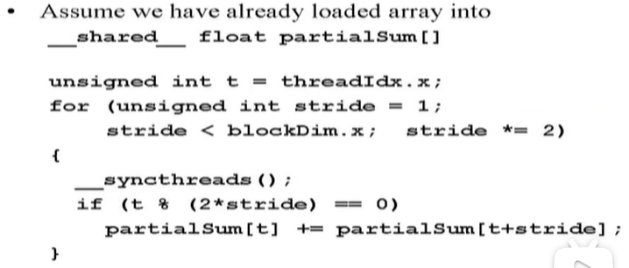
\includegraphics[width=3in]{code1.png}
    \end{minipage}
}
\subfigure[]{
    \begin{minipage}[t]{0.4\linewidth}
    \centering
    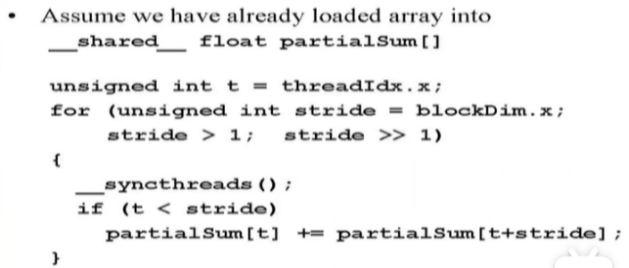
\includegraphics[width=3in]{code2.png}
    \end{minipage}
}
\end{figure}
~\\
Ans:%input your answer here
~\\
~\\Parallel reduction refers to algorithms which combine an array of elements producing a single value as a result.
~\\The first: 1=1+2, 3=3+4..., then 1=1+3, 5=5+7..., then....\\The second: 1=1+stride, 2=2+stride..., then stride/2, then 1=1+stride, 2=2+strid.
~\\The second is better.Because all the number next to the number do together, but the first the next number haven't do operation, only the number far away do, it will cost time.
\section{What are TLP and ILP? How to improve ILP? Why do we need to avoid writing programs that have dependencies like the below? (no more than 100 words)}
\qquad \quad c = a + b;

\qquad \quad d = c + a;

Ans:%input your answer here
~\\TLP is Short for thread-level parallelism.
~\\Instruction-level parallelism (ILP) is a measure of how many of the instructions in a computer program can be executed simultaneously.
~\\Because the d = c + a, the d will need the c, that is the second operation need the result of the first operation, it can't do that using parallel well, costs many time.
\section{What arrays does CSR have? What other storage formats does a sparse matrix have? Please draw a 4×4 dense matrix with some zeros and covert it to the CSR format. You are asked to attach a figure. (no more than 50 words)}

Ans:%input your answer here
\\CSR has three arrays: Indicates the index of the beginning and end of each row of data in the matrix, Indicates the number of columns and rows of the corresponding data in data in the matrix, than is the number in matris(not 0).\\
\\COO, coordinate format.\\
CSR, compressed sparse row format.\\
MSR, modified sparse row format.\\
CSC, compressed sparse column format.\\
MSC, modified sparse column format.\\
DIA, the diagonal sparse matrix format (NOT a diagonal matrix!).\\
DIAG, a diagonal matrix, stored as a vector.\\
LNK, linked storage format.\\
BSR, block row sparse format.\\
DOK,Dictionary of keys\\
BND, the LINPACK format for general banded matrices.\\
ELL, ELLPACK/ITPACK, the format used by ELLPACK and ITPACK.\\
HB, Harwell-Boeing format. (Actually, CSR format plus auxilliary data)\\
JAD, the jagged diagonal format.\\
SSK, Symmetric skyline format.\\
SSR, Symmetric sparse row format.\\
\\The picture is at the end.

%upload your photo and insert it

\begin{figure}[ht!]
\centering

\includegraphics[width=5in]{example}
%\caption{example}
\end{figure}

\section{List the best speedups you observed while you compared the performance of the vector-version and the scalar-version of SpMM with CUDA. Consider your hardware environment of the machine and the size of the problem. And why is the vector-version faster than the scalar-version? If the scalar-version is faster, please analyze your performance data. (no more than 200 words)}

Ans:%input your answer here
~\\The scalar:\\
harvest7 = np.array([[0.00004, 0.00013, 0.00028, 0.00051, 0.00077, 0.00119, 0.00154, 0.00200, 0.00262, 0.00320, 0.00372, 0.00443, 0.00499, 0.00581, 0.00656, 0.00734, 0.00840, 0.00937, 0.01040, 0.01155],
[0.00008, 0.00024, 0.00055, 0.00100, 0.00154, 0.00235, 0.00306, 0.00398, 0.00488, 0.00597, 0.00690, 0.00832, 0.00961, 0.01122, 0.01290, 0.01472, 0.01621, 0.01817, 0.02038, 0.02285],
[0.00015, 0.00048, 0.00110, 0.00200, 0.00307, 0.00461, 0.00569, 0.00739, 0.00961, 0.01153, 0.01366, 0.01666, 0.01933, 0.02254, 0.02542, 0.02916, 0.03261, 0.03638, 0.04076, 0.04569]])
\\The vector:\\
harvest8 = np.array([[0.00001, 0.00003, 0.00005, 0.00009, 0.00013, 0.00022, 0.00026, 0.00034, 0.00047, 0.00057, 0.00063, 0.00075, 0.00091, 0.00103, 0.00109, 0.00125, 0.00153, 0.00166, 0.00176, 0.00200], 
[0.00002, 0.00004, 0.00009, 0.00016, 0.00025, 0.00039, 0.00050, 0.00067, 0.00082, 0.00104, 0.00113, 0.00141, 0.00164, 0.00194, 0.00216, 0.00251, 0.00279, 0.00319, 0.00352, 0.00397], 
[0.00003, 0.00008, 0.00018, 0.00032, 0.00051, 0.00074, 0.00092, 0.00121, 0.00155, 0.00191, 0.00224, 0.00277, 0.00325, 0.00380, 0.00429, 0.00494, 0.00555, 0.00623, 0.00695, 0.00786]]) 
\\The vector is faster.
\bibliographystyle{plain}
\end{document}
